\فصل{تصویرسازی سامانه‌ها}
در فصل‌های گذشته تنها با ثبت عددی خروجی‌های مدلسازی سروکار داشتیم. خروجی‌ها تلاش داشتند تا رفتار سامانه را به ما بشناسانند. ما نیز تلاش کردیم تا بررسی اشکال و نمودارها آنچه را که در پس‌پرده [جعبه سیاه] می‌گذرد؛ «حدس» بزنیم. به همین دلیل برآن شدیم تا روشی برای به تصویر کشیدن سامانه ابداع کنیم تا از لحظه‌لحظه‌ی سامانه با خبر شویم. شکل \ref{fig:if_animation_plot}

\begin{figure}[h]
	\centering
	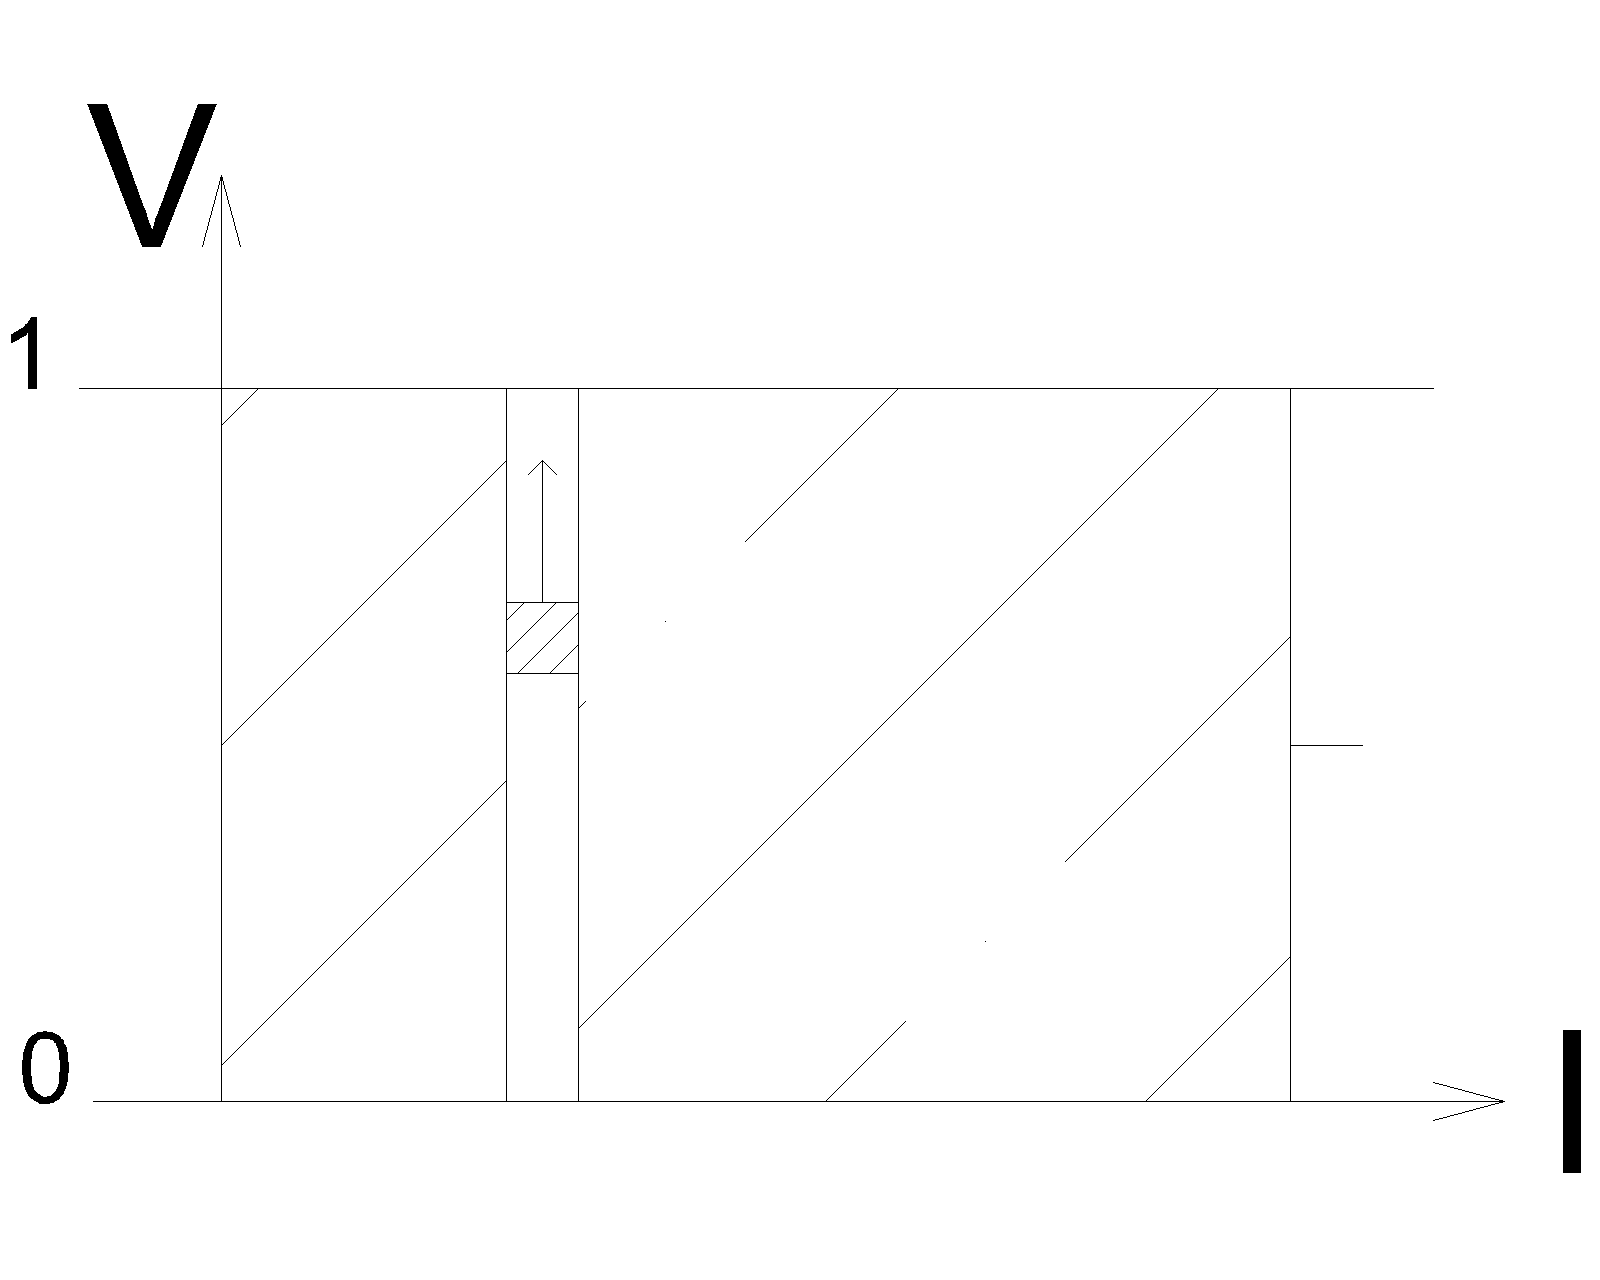
\includegraphics[width =0.8\textwidth]{../papers_studies/figs/IF/IF_phase_space-Model.png}
	\caption{تصویر فضای فاز سامانه نورونی انباشت‌وشلیک}
	\label{fig:if_animation_plot}
\end{figure}

پویایی شکل \ref{fig:if_animation_plot} به ما نشان خواهد داد که چگونه سامانه در زمان متحول می‌شود. هر نقطه در این صفحه نمایانگر حالت یک نورون است. محور افقی نشان دهنده‌ی جریان ثابت خارجی است که به هر نورون در ابتدا متصل کرده‌ایم و محور عمودی نشان دهنده‌ی پتانسیل نورون است.طبق توصیفی که از پویایی سامانه‌ی خود داریم؛ توقع داریم که نورون‌هایی که از آستانه عبور کردند؛ مجددا از محور صفر پیدا شوند.\\

حال 